\documentclass[12pt]{article}
\usepackage[utf8]{inputenc}
\usepackage[style=apa, backend=biber]{biblatex} 
\DeclareLanguageMapping{american}{american-apa}
\addbibresource{references.bib}
\usepackage{csquotes, geometry, graphicx, setspace, xcolor, url, footmisc, fancyhdr}
\geometry{margin=1in}
\doublespacing
\setlength{\parskip}{1em}
\definecolor{kingcolor}{rgb}{0.5,0,0.5}
\definecolor{douglasscolor}{rgb}{0,0,1}
\pagestyle{fancy}
\fancyhf{}
% Running header with last name and page number
\fancyhead[R]{Vaught \thepage}

\begin{document}

% MLA Heading
\noindent J.C. Vaught\\
Dr. Nancy Tolson\\
AFAM 200

The silence was unnerving. The heavy air inside the church seemed to breathe on its own, filling the space with a faint yet distinct mechanical hum, as if the walls themselves held a secret they dared not speak aloud. The stained-glass windows cast eerie, shifting patterns of light onto the perfectly polished mahogany pews, each colored beam painting ghastly trails on the dusty floor. Dr. King opened his eyes and immediately felt the weight of something unexplainable. He didn’t remember how he arrived; one moment he felt the weight of his work on his shoulders, the next, a strange, oppressive silence had taken its place. The disorienting shift left him unsettled, as though the ground had been swept out from beneath him, and he was suspended in a liminal space.

\begin{figure}[h]
  \centering
  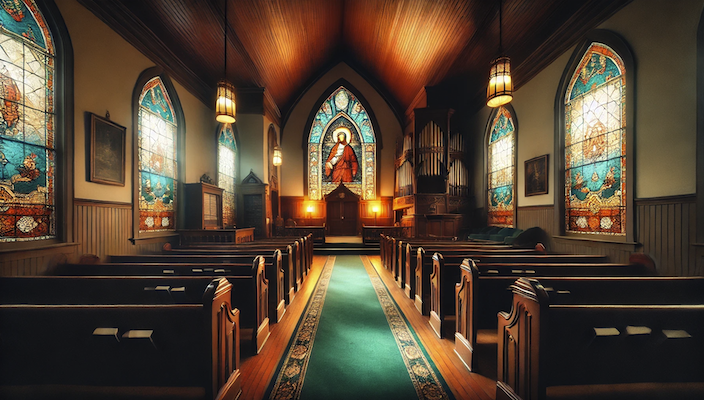
\includegraphics[width=0.7\linewidth]{church.png}
  \caption{A traditional church}
  \label{fig:church}
\end{figure}

Across the room, another figure stirred. Frederick Douglass sat upright, his piercing eyes scanning the strange surroundings. Neither man spoke at first, both acutely aware that they were not alone but wholly uncertain of where, or when, they might be. The rustling of leaves outside was the only audible sound, interrupted by the faint creak of the building settling on its foundation. A voice finally broke the silence.

{\color{kingcolor}``Who are you? Where am I?''} King's voice, normally rich with authority yet now edged in unease, filled the hallowed space. He took a cautious step forward, the faint echo of his shoes penetrating the oppressive silence, {\color{kingcolor}``And what is this place?''}

Douglass’s sharp gaze locked onto King. {\color{douglasscolor}``I was about to ask you the same. It seems we are two souls in this chapel. Tell me, are you a man of the living or something else entirely?''} His words were deliberate, edged with suspicion. 

{\color{kingcolor}``A man of the living, I assure you,''} King replied, straightening his posture. {\color{kingcolor}``Dr. Martin Luther King Jr., at your service. And you, sir? Your presence feels almost... historic.''} The last word lingering in the silence as if an accusation.

With a faint smile that hinted at pride, Douglass replied with a chuckle, {\color{douglasscolor}``Historic, perhaps, though I have never been called such before. I am Frederick Douglass, born a slave, but I refused to die one. And you, Dr. King, do you fight as I once fought?''}

King’s breath caught. {\color{kingcolor}``The Frederick Douglass?''} His voice trembled with a profound reverence. {\color{kingcolor}``I have read your works; your words shaped the foundations of freedom in my country. But yes, I fight, though not with chains or rifles, but with marches and words. Our enemies are no longer slave owners but segregationists. And you? How did you come to be here?''}

{\color{douglasscolor}``I wish I knew. One moment, I was preparing to address a crowd, emboldened by Lincoln’s proclamation. The next, I awaken here, in a place that feels like it knows our names before we do.''} Douglass glanced around, his tone growing darker. {\color{douglasscolor}``Perhaps we have been summoned to reconcile our battles... or our failures.''}

{\color{kingcolor}``Failures?''} King stepped closer, his voice rising. {\color{kingcolor}``Mr. Douglass, your struggle paved the way for my own. You turned a tide of ignorance into a wave of liberation. Failures? No, your legacy is anything but.''}

\bigskip
\subsection*{DIALOGUE}


Douglass held up a hand. {\color{douglasscolor}``You misunderstand me, Dr. King. I do not speak of personal failures but of humanity’s. Tell me, after all I fought for, does the Negro stand free and equal in your time? Or does he still endure beneath new shackles?''}

King exhaled slowly, his expression pained. {\color{kingcolor}``The chains are different, but they bind all the same. I have seen children turned away from schools, families denied homes, and men beaten for daring to vote and engage in their political system. The enemy now hides behind laws and customs, but his intent remains cruelly familiar.''}

{\color{douglasscolor}``Then it seems we share more than I would have hoped.''} Douglass’s voice hardened. {\color{douglasscolor}``Tell me, Dr. King, how do you resist the urge to strike back? To show the oppressor the strength of a people who will not be trampled?''}

King’s expression softened, though his eyes held steady. {\color{kingcolor}``Mr. Douglass, I teach that nonviolence is not weakness, but strength. It is a conscious decision to meet oppression with dignity. As I have often said, 'Nonviolence is a powerful and just weapon. It is a sword that heals' \parencite{king1963letter}.''}

Douglass raised an eyebrow, intrigued. {\color{douglasscolor}``A sword that heals, you say? And does it cut deep enough to draw the blood of justice? Do you \textit{truly} believe your enemy can be moved without fear of reprisal?''}

King’s face darkened momentarily, his voice heavy with frustration. {\color{kingcolor}``I confess there are days when the devil's anger tempts me. When I think of my children, when I see the tears in my daughter’s eyes because she cannot go to an amusement park, or hear my son ask why white people treat us so cruelly, my heart burns with rage. And yet, I know this: to yield to hate is to become what we abhor. The moderates who tell me to `wait,' who value peace over justice, who caution patience while we suffer - they enrage me. But their hearts, hardened by complacency, will not be softened by violence.''}

Douglass’s laugh was low and bitter. {\color{douglasscolor}``You speak of light to men who dwell in darkness. I have faced these same moderates, those who claimed to abhor slavery yet did nothing to end it. `Power concedes nothing without a demand,' I once said, but I will add this: it concedes even less to silence. The hypocrisy of these men to fight for freedom yet enslave others is astounding.\parencite{douglass1852fourth}''}

{\color{kingcolor}``And yet, Mr. Douglass, it is not just the moderate who fails us, but the very structure they cling to. The white man’s illusion of time, that progress will come if we only wait, is the lie that keeps justice at bay. As I wrote, `This ``Wait" has almost always meant ``Never."'\newline
If only they could see the world through my children’s eyes, perhaps their hearts would soften.''}

Douglass’s tone grew sharper, frustration bleeding through his composed demeanor. {\color{douglasscolor}``Soften their hearts? Dr. King, more than a \textit{century} separates my fight from yours, yet their hearts remain as unyielding as stone. Do you realize what that means?! More time has passed between my struggle and yours than between the founding of this nation and the abolition of slavery. And still yet, the Negro suffers indignities that mock the very notion of freedom! How can we speak of \textit{progress} when history seems content to repeat its cruelties, as if it has learned nothing from the blood that was spilled?''}

King’s voice rose with quiet intensity, a deep well of sorrow evident in his tone. {\color{kingcolor}``Perhaps it is, Mr. Douglass. But what choice do we have but to hope, to fight? If I must burn, let it be as a beacon, not a blaze of destruction. The ashes of hatred leave no foundation for the world my children deserve. I too feel the weight of time’s cruel march; Every year that passes feels like another betrayal of justice, another debt unpaid. The promises of freedom ring hollow when my children cannot play where they wish, when families are told they are less than human, when men are brutalized for daring to vote. My hope lies in breaking this cycle, not simply by waiting, but by forcing the world to see our humanity.''}

Douglass’s jaw tightened, his frustration mingling with a cold fury. {\color{douglasscolor}``And if they refuse to see? If they harden their hearts further? If the lessons of the past fall on deaf ears, as they so often do? I’ve seen this all before. Men who claim to be allies but will not risk their comfort; leaders who promise change but deliver chains. History has taught me that fire is often the only light that men will see. It burns away the lies, the illusions, and leaves them with nothing but the truth.''}

King stepped closer, his voice calm but resolute. {\color{kingcolor}``And yet, Mr. Douglass, fire consumes indiscriminately. If we destroy everything, what remains to build upon? I too feel the anger, the temptation to meet their hate with equal force. But if we are to claim the moral high ground, to show them a better way, then we cannot succumb to their methods. As I have said, `Returning hate for hate multiplies hate. Darkness cannot drive out darkness; only light can do that.' \parencite{king1963letter}''}

Douglass paused, his expression softening slightly as he studied King. {\color{douglasscolor}``Perhaps we are simply two sides of the same coin. Your light and my fire, they both seek to illuminate a path forward. But tell me, does your faith not falter when the years stretch on and the progress feels so meager? How do you reconcile a godly vision with the unrelenting cruelty of men?''}

King’s voice deepened with solemn conviction. {\color{kingcolor}``It is my belief that God’s justice is not bound by the failings of man. As I have said, `The arc of the moral universe is long, but it bends toward justice.' It is not for us to dictate the timeline of divine will, but to remain steadfast in our purpose. Even in despair, we must trust in God’s greater plan.''}

Douglass’s gaze darkened as he stepped closer. {\color{douglasscolor}``But does it not anger you that we are forced to appeal to their better angels when history has shown so few of them exist? That we must endure their `wait' while they crush the spirit of your children and mine? Tell me, how do you temper that fury?''}

King looked away briefly, his voice trembling with emotion. {\color{kingcolor}``I temper it with love, Mr. Douglass, though at times it feels impossible. My children, my son and daughter, they are growing up in a world that teaches them to doubt the goodness of man. And yet, I tell them to love. To love a world that does not yet love them back. It is the greatest challenge of my faith, but it is also its greatest command.''}

Douglass’s voice grew cold, each word deliberate. {\color{douglasscolor}``Then perhaps it is God’s justice we must invoke - for man’s justice is a phantom. But let me ask you this: when the final reckoning comes, will they answer for the centuries of blood, the endless cries of the oppressed? Or will history grant them its usual absolution?''}

Before King could answer, the faint hum in the air deepened into an unsettling vibration, rattling the stained-glass windows. The colors distorted, the once-reassuring patterns twisting into something almost menacing. 

King’s gaze snapped back to Douglass, urgency sharpening his tone. {\color{kingcolor}``They will answer, Mr. Douglass. If not in this life, then in the next. But it is not for us to mete out that judgment. Ours is to fight, to struggle, to strive for a better world, knowing that even if we fail, we have done so with righteousness in our hearts. That is the legacy I wish to leave my children: not vengeance, but a vision of the kingdom of God on earth.''}

The hum grew louder; a crack appeared in the largest stained-glass window, running through the image of Jesus being crowned with the biblical crown of thorns.

Douglass’s lips curled into a faint, bitter smile as his eyes darted to the shattering glass. {\color{douglasscolor} ``A vision, you say. Perhaps that is what separates us. You cling to vision; I to memory. But let me leave you with this, Dr. King; if God’s justice delays, perhaps it is because \textbf{He waits for men to earn it}."}


\printbibliography
\end{document}
